\chapter{Filterung von Signalen}
Die Frequenz Filterung von Signalreihen kann bestimmte Eigenschaften von Signalen hervorheben als auch Störende Signale (\textit{Noise}) entfernen.\\
Beim picken von Ersteinsätzen sollte die kausale Filterung angewendet werden.

\section{Zweiseitige Filterung} 
In Matlab wird es mit dem Befehl filtfilt durchgeführt.\\
Folgende Schritte stecken hinter dem Befehl filtfilt.
\begin{enumerate}
\item Filterung von links nach rechts:
\begin{equation}
Y(\omega) = F(\omega)X(\omega)
\end{equation}
In Matlab wird dafür das Befehl filter verwendet. \\
\item Umkehrung der Zeitachse, Filterung rechts nach links. Somit erfolgt eine Spiegelung und Verschiebung.
\begin{equation}
y_{r} = y(T-t)
\end{equation}
Danach filtert man von links nach rechts:
\begin{equation}
y_{r}(\omega) = \exp^{-i\omega t} y^*(\omega) 
\end{equation}
Dabei ist $y^*(\omega)$ das Komplexkonjugierte von $y(t)$.\\
\item Schritt: Eine erneute Filterung erfolgt: $z_{r}= F(\omega)y_{r}(\omega)$\\
\item Schritt: Umgehung der Zeitachse :
\begin{equation}
z(t)=z_{r}(T-t)
\end{equation}

\begin{equation}
z(\omega)=\exp^{-i\omega T}z_{r}^*(\omega) = \exp^{-i\omega T} F^*(\omega) \exp^{-i\omega T} F(\omega)X(\omega)
\end{equation}
Das ergibt ein sehr einfaches Ergebnis:
\begin{equation}
z(\omega)=   F^*(\omega) F(\omega)X(\omega) = \vert F(\omega) \vert^2 X(\omega)
\end{equation}

Dabei ist $\vert F(\omega) \vert^2$  die nullphasige Filterung. Die Flanken werden schärfer, das ermöglicht die Anwendung von filtfilt in Matlab.
\end{enumerate}

\section{f-k-Filterung}
Mit Hilfe der 2D-Fouriertransformation: $u(x,t)\longrightarrow u(k,\omega)$\\
Dann definiert man die minimale und maximale Durchlassgeschwindigkeit. Man filtert mit den Grenzen: \\
\begin{equation*}
\dfrac{\omega}{c_{max}}\leq k(\omega)\leq \frac{\omega}{c_{min}}
\end{equation*}
Dieser Filter wird angewendet, um z.B. die Oberflächenwellen zu unterdrücken und um die Reflexionen der Raumwellen besser zu sehen.

\section{Tiefpassfilter}
Abbildung \ref{fig:filt_tiefpass} zeigt den Verlauf der Ausgangsspannung $U_a$ eines Tiefpasses in Abhängigkeit der Frequenz. Signale mit Frequenzen unterhalb der Grenzfrequenz $f_g$ gelten als durchgelassene Signale. Signale mit Frequenzen oberhalb der Grenzfrequenz $f_g$ gelten als gesperrte Signale.\\
\begin{figure}[h!]
\centering
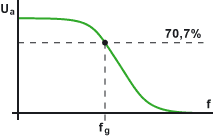
\includegraphics[width=.4\tw]{fig/06-Filter/tiefpass.png}
\caption{Darstellung eines Tiefpassfilters im Frequenzbereich.}
\label{fig:filt_tiefpass}
\end{figure}
Der Durchlassbereich ist der Bereich in dem gilt : $\vert F(\omega) \vert \approx 1 $.
Im Sperrbereich gilt: $\vert F(\omega) \vert \approx 0 $. Wo die Amplitude auf: 
$20log(0,7079)dB \approx 3dB$,  abklingt, dort ist die Eckfrequenz.

\section{Hochpassfilter}
Beim Hochpassfilter werden die Frequenzen bis zu einer bestimmten Frequenz $\omega_{h}$  gesperrt. Frequenzen ab dieser Frequenz $\omega_{h}$ werden durchgelassen.
\begin{figure}[h!]
\centering
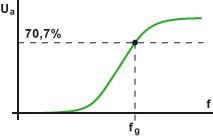
\includegraphics[width=.4\tw]{fig/06-Filter/hochpass.png}
\caption{Darstellung eines Hochpassfilters im Frequenzbereich.}
\end{figure}

\section{Bandpassfilter}
Der Durchlassbereich liegt zwischen den Frequenzen $\omega_{1}$ und $\omega_{2}$. \\
$\vert F(\omega) \vert \approx 1 $ für $\omega_{1} \ll\omega \ll\omega_{2}$. Abbildung \ref{fig:filt_bandpass} zeigt den Bandpassfilter für die Frequenz um 440 Hz. 
\begin{figure}[h!]
\centering
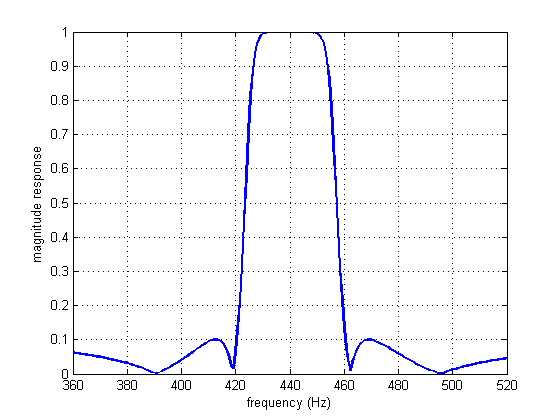
\includegraphics[width=.4\tw]{fig/06-Filter/bandpass.png}
\caption{Darstellung eines Bandpassfilters im Frequenzbereich.}
\label{fig:filt_bandpass}
\end{figure}

\section{Akkusaler Tiefpassfilter}
Beim akkusalen Tiefpassfilter handelt es sich um ein Boxcar. 
\begin{figure}[h!]
\centering
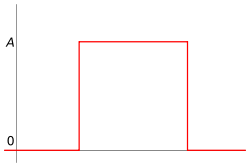
\includegraphics[width=.6\tw]{fig/06-Filter/boxcar.png}
\caption{Darstellung eines akausalen Tiefpassfilters im Frequenzbereich.}
\end{figure}